\documentclass[11pt,a4paper]{article}
\usepackage{gtu-el-yazisi}
\begin{document}
\notbilgi{Nümerik Analiz}{3. Ders -- Kök bulma yöntemleri (devamı): Newton, sekant ve hata analizi}{numerik-3.ders.pdf}

\sayfa{1}
\noindent\textit{3. ders}

\section{Kök bulma yöntemleri -- devamı}
\subsection{Newton (Newton-Raphson) yöntemi}
$f:[a,b]\to\mathbb{R}$ için $f(x)=0$, \ $x=p$ kökünü sayısal olarak bulalım

$f\in C^2[a,b]$ ve $p_0\in[a,b]$ bir nokta

$f'(p_0)\neq 0$ ve $|p-p_0|$ küçük bir büyüklük

\medskip
\noindent{\small\textit{lineer taylor polinomu}} \ $=$
\[
  f(x)=f(p_0)+f'(p_0)\,(x-p_0)+\frac{f''(\xi)}{2!}\,(x-p_0)^2 \qquad\qquad (p-p_0)^2\cong 0
\]
\[
  0=f(p_0)+f'(p_0)\,(p-p_0)+\frac{f''(\xi)}{2!}\,(p-p_0)^2
\]
\[ p\cong p_0-\frac{f(p_0)}{f'(p_0)}=p_1 \]
$p_n$, \ $n=1,2,\dots$
\[
  p_n=p_{n-1}-\frac{f(p_{n-1})}{f'(p_{n-1})}\ , \qquad n=1,2,\dots
\]

\noindent\begin{minipage}[c]{0.6\linewidth}
\centering
\begin{tikzpicture}[murekkep,line width=0.7pt,x=1cm,y=1.1cm]
  \draw[->] (0,0) -- (5.6,0);
  \draw[->] (0.6,-1.35) -- (0.6,1.5);
  \draw[domain=0.9:5.4,samples=80,smooth] plot (\x,{1.2*tanh((\x-3)/1.6)});
  \draw[kursunkalem] (0.9,-1.0714) -- (5.0,0.22);
  \draw[kursunkalem] (2.0,-0.1423) -- (5.0,1.0934);
  \draw[dashed,kursunkalem] (1.4,0) -- (1.4,-0.9139);
  \draw[dashed,kursunkalem] (4.3015,0) -- (4.3015,0.8057);
  \fill (1.4,0) circle (1.2pt) node[above left] {$p_0$};
  \fill (2.3455,0) circle (1.2pt) node[above] {$p_2$};
  \fill (3,0) circle (1.2pt) node[below right] {$p$};
  \fill (4.3015,0) circle (1.2pt) node[above left] {$p_1$};
  \fill (1.4,-0.9139) circle (1.2pt) node[below] {$f(p_0)$};
  \fill (4.3015,0.8057) circle (1.2pt) node[above] {$f(p_1)$};
  \draw (4.75,0) arc (0:22:0.45);
  \node[below] at (4.75,-0.02) {$\alpha$};
\end{tikzpicture}
\end{minipage}\hfill
\begin{minipage}[c]{0.38\linewidth}
\[ \tan\alpha=f'(p_0) \]
\[ \tan(\pi-\alpha)=-f'(p_0)\neq0 \]
\end{minipage}

\begin{ornek}
$[0,\pi/2]$ \quad $f(x)=\cos x-x$ \qquad $f(x)=0$ denkleminin kökünü
\begin{enumerate}[label=\alph*)]
  \item $p_0=\frac{\pi}{2}$ alıp sabit nokta iterasyonuyla $p_6$'yı
  \item $p_0=\frac{\pi}{2}$ Newton ile $n=1,2,3$ uygulayarak $p_3$'ü bulunuz
\end{enumerate}
\end{ornek}
\[ \cos x-x=0 \]
\[ g(x)=\cos x=x \]
a)\quad $g(x)=\cos x$ \qquad $p_n=g(p_{n-1})$ \quad $n=1,2,\dots$
\begin{align*}
  &p_1=\cos\left(\tfrac{\pi}{2}\right)=0,\quad p_2=\cos(0)=1,\quad p_3=\cos(1)\cong0{,}540302\\
  &p_4=\cos(p_3)\cong0{,}8575532,\quad p_5=\cos(p_4)\cong0{,}6542898\\
  &p_6=\cos(p_5)\cong0{,}7934805
\end{align*}
\[
  p_n=p_{n-1}-\frac{\cos(p_{n-1})-p_{n-1}}{-\sin(p_{n-1})-1}
     =p_{n-1}+\frac{\cos p_{n-1}-p_{n-1}}{\sin p_{n-1}+1}
\]

\sayfa{2}
b)
\begin{align*}
  p_1&=p_0+\frac{\cos p_0-p_0}{\sin p_0+1}=\frac{\pi}{2}+\frac{-\pi/2}{2}=\frac{\pi}{4}\\[1mm]
  p_2&=p_1+\frac{\cos p_1-p_1}{\sin p_1+1}=\frac{\pi}{4}+\frac{\frac{1}{\sqrt2}-\frac{\pi}{4}}{1+\frac{1}{\sqrt2}}\cong0{,}7395361\\[1mm]
  p_3&=p_2+\frac{\cos p_2-p_2}{\sin p_2+1}\cong0{,}7956852\footnotemark
\end{align*}
\footnotetext{Claude notu: muhtemelen $p_3\cong0{,}7390852$ olmalı.}

\begin{teorem}[1]
$f\in C^2[a,b]$, Eğer $p\in[a,b]$ noktasında $f(p)=0$ ve $f'(p)\neq0$ olursa o halde öyle bir
$\delta>0$ vardır ki, Newton iterasyonu her $p_0\in[p-\delta,\,p+\delta]$ başlangıç iterasyonu için
$p$ sayısına yakınsar.

\hfill
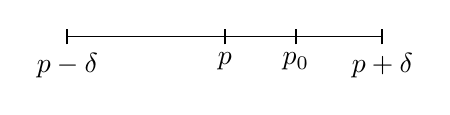
\begin{tikzpicture}[line width=0.7pt]
  \draw (0,0) -- (4,0);
  \foreach \x/\l in {0/p-\delta,2/p,2.9/p_0,4/p+\delta} {\draw (\x,-0.1) -- (\x,0.1); \node[below] at (\x,-0.08) {$\l$};}
\end{tikzpicture}
\end{teorem}

\subsection{Sekant yöntemi}
\[
  f'(p_{n-1})=\lim_{x\to p_{n-1}}\frac{f(x)-f(p_{n-1})}{x-p_{n-1}}\ \Bigg|\
  \approx\ \frac{f(p_{n-2})-f(p_{n-1})}{p_{n-2}-p_{n-1}}
\]
\hspace*{6.5cm}{\small $p_{n-2}$ çok yakın $p_{n-1}$}
\[
  =\frac{f(p_{n-1})-f(p_{n-2})}{p_{n-1}-p_{n-2}}
\]
\[
  p_n=p_{n-1}-\frac{f(p_{n-1})\,(p_{n-1}-p_{n-2})}{f(p_{n-1})-f(p_{n-2})}\ , \qquad n=2,3,\dots
\]

\begin{ornek}[2]
$p_0$ ve $p_1$ başlangıç iterasyonlarına gereksinim duyuyor!

$f(x)=x^2-6$
\begin{enumerate}[label=\alph*)]
  \item $p_0=1$ $\rightarrow$ $p_2$'yi Newton Y. ile bulun
  \item $p_0=3$, $p_1=2$; $p_3$'ü Sekant y. ile bulun
\end{enumerate}
\end{ornek}
\[ f'(x)=2x \]
a)\quad NI: \ $p_n=p_{n-1}-\dfrac{p_{n-1}^2-6}{2p_{n-1}}$ \qquad $n=1,2,\dots$
\[
  p_1=p_0-\frac{p_0^2-6}{2p_0}=1-\frac{1-6}{2}=\frac72\ ;\qquad
  p_2=\frac72-\frac{\left(\frac72\right)^2-6}{2\cdot\frac72}=\frac{73}{28}\cong2{,}607143
\]
b)\quad Sekant yöntemi
\begin{align*}
  p_n&=p_{n-1}-\frac{(p_{n-1}^2-6)\,(p_{n-1}-p_{n-2})}{p_{n-1}^2-p_{n-2}^2}\\
     &=p_{n-1}-\frac{p_{n-1}^2-6}{p_{n-1}+p_{n-2}}
\end{align*}

\sayfa{3}
\[ p_2=\frac{12}{5} \]
\[ p_3=\frac{p_1p_2+6}{p_1+p_2}\cong2{,}454545 \]

\subsection{İterasyon yöntemlerinde Hata analizi}
\begin{tanim}
$p_n$, $n=1,2,3,\dots$ dizisi $p_n\neq p$ olacak biçimde $p$'ye yakınsak bir dizi olsun. Eğer;
\[ \lim_{n\to\infty}\frac{|p_{n+1}-p|}{|p_n-p|^{\alpha}}=\lambda \]
olacak şekilde $\lambda$ ve $\alpha$ sayıları bulunabiliyorsa; $p_n$, $n=1,2,3$, dizisi
``asimtotik hata sabiti $\lambda$ olacak biçimde $p$ sayısına $\alpha$'ıncı dereceden yakınsaktır.''
\end{tanim}

\noindent\begin{minipage}[c]{0.3\linewidth}
\begin{tikzpicture}[line width=0.6pt,murekkep]
  \node (p) at (0,0) {$p_n$};
  \draw[->] (p.east) -- ++(0.5,0.4) node[right] {ikiye bölme};
  \draw[->] (p.east) -- ++(0.5,0) node[right] {Sekant};
  \draw[->] (p.east) -- ++(0.5,-0.4) node[right] {Newton};
\end{tikzpicture}
\end{minipage}

\begin{tabular}{@{}lll}
  $\alpha=1$ & ``Lineer yakınsak'' & \\
  $\alpha=2$ & ``kuadratik yakınsak'' & \\
  $\alpha=3$ & ``kübik \quad '' \quad ''
\end{tabular}

\medskip
\noindent\begin{minipage}[c]{0.6\linewidth}
\[ \lim_{n\to\infty}\frac{|p_{n+1}|}{|p_n|}=0{,}5 \quad\text{olsun} \]
\[ \lim_{n\to\infty}\frac{|q_{n+1}|}{|q_n|^2}=0{,}5 \]
\end{minipage}\hfill
\begin{minipage}[c]{0.36\linewidth}
$p_n\to0$'a yakınsak\\ \hspace*{1em}$n=1,2,\dots$

\medskip
$q_n\to0$\\ \hspace*{1em}$n=1,2,\dots$
\end{minipage}
\begin{align*}
  \frac{|p_{n+1}|}{|p_n|}\approx0{,}5 \ &\Rightarrow\ |p_n|\approx0{,}5\,|p_{n-1}|\approx(0{,}5)^2\,|p_{n-2}|
     \approx\dots\approx\kutula{(0{,}5)^n}\,|p_0|\\
  \frac{|q_{n+1}|}{|q_n|^2}\approx0{,}5 \ &\Rightarrow\ |q_n|\approx0{,}5\,|q_{n-1}|^2=0{,}5\left[0{,}5\,|q_{n-2}|^2\right]^2\\
  &\approx(0{,}5)^3\,|q_{n-2}|^4\approx\dots\approx\kutula{(0{,}5)^{2^n-1}}\,|q_0|^{2^n}
\end{align*}
\begin{center}
\begin{tabular}{ccc}
  & $\alpha=1,\ p_0=1$ & $\alpha=2,\ q_0=1$\\
  $n$ & $p_n=(0{,}5)^n$ & $q_n=(0{,}5)^{2^n-1}$\\ \midrule
  1 & 0,5 & 0,5\\
  2 & 0,25 & 0,125\\
  3 & 0,125 & 0,0078125\\
  4 & 0,0625 & 0,000030518\\
  5 & 0,03125 & $0{,}46566\cdot10^{-9}$\\
  6 & 0,015625 & $0{,}10842\cdot10^{-18}$
\end{tabular}
\end{center}

\sayfa{4}
\begin{ornek}
\begin{enumerate}[label=\arabic*)]
  \item $p_n=10^{-2^n}$ \quad $n=1,2,\dots$ dizisi 0'a kuad. yakınsar mı
  \item $p_n=10^{-n^2}$, \quad $n=1,2$ \quad '' \qquad '' \qquad ''
\end{enumerate}
\end{ornek}
\noindent\begin{minipage}[c]{0.7\linewidth}
\[
  1)\quad \frac{|p_{n+1}|}{|p_n|^2}=\frac{10^{-2^{n+1}}}{\left(10^{-2^n}\right)^2}=\frac{10^{-2^{n+1}}}{10^{-2^{n+1}}}=1
\]
\end{minipage}\hfill
\begin{minipage}[c]{0.28\linewidth}
yakınsaktır (sabit sayı çıktığından)
\end{minipage}
\[
  2)\quad \frac{|p_{n+1}|}{|p_n|^2}=\frac{10^{-(n+1)^2}}{\left(10^{-n^2}\right)^2}=\frac{10^{-(n+1)^2}}{10^{-2n^2}}
  =10^{-(n^2+2n+1)+2n^2}
\]
\[
  =10^{n^2-2n-1} \quad \text{\large$\times$}\ \text{sabit değil}
\]
\[ \lim_{n\to\infty}\frac{|p_{n+1}|}{|p_n|^2}\to\infty \]

\begin{teorem}[2]
$g\in C[a,b]$ ve her $x\in[a,b]$ için $g(x)\in[a,b]$. Ayrıca $(a,b)$'de $g'$ türevi sürekli mevcut
öyle ki; $|g'(x)|\le k$ ; $k<1$ biçiminde $k$ mevcut olsun. Eğer $g'(p)\neq0$ olursa $\rightarrow$
$p_0\in[a,b]$, $p_0\neq p$ başlangıç iterasyonu için $p_n=g(p_{n-1})$ $n=1,2,\dots$ Sabit nokta
iterasyonu $p\in[a,b]$ sabit noktasına lineer yakınsar.
\end{teorem}

\textbf{İspat}\quad Sab. Nokta teor. $\Rightarrow$ $p_n\to p$ \ $(n\to\infty)$
\[
  p_{n+1}=g(p_n) \qquad\qquad p=g(p)\ \Rightarrow\ p_{n+1}-p=g(p_n)-g(p)
\]
ortalama değer teoremi $\Rightarrow$ \quad $=g'(\xi_n)\,(p_n-p)$
\[ \frac{|p_{n+1}-p|}{|p_n-p|}=|g'(\xi_n)| \]
\[
  \rightarrow\ \lim_{n\to\infty}\frac{|p_{n+1}-p|}{|p_n-p|}=\lim_{n\to\infty}|g'(\xi_n)|=|g'(p)|\neq0
\]

\begin{teorem}[3]
$p$ sayısı $x=g(x)$ denkleminin çözümü olsun. Ayrıca $g'(p)=0$ ve $p$'yi içeren bir $I$ aralığında
sürekli $g''$ türevi mevcut olsun öyleki $|g''(x)|<M$ sağlansın. Bu durumda öyle bir $\delta>0$ sayısı
mevcut olurki, her $p_0\in[p-\delta,\,p+\delta]$ başlangıç iterasyonu için $p_n=g(p_{n-1})$
iterasyonu $p$'ye quadratik yakınsak. Ayrıca keyfi büyük $n$ sayılar için,
$|p_{n+1}-p|<\dfrac{M}{2}\,|p_n-p|^2$ sağlanır.

\[ \kutula{\begin{aligned} g(p)&=p\\ g'(p)&=0 \end{aligned}} \]
\end{teorem}

\sayfa{5}
\noindent\begin{minipage}[c]{0.68\linewidth}
\[ f(x)=0 \ \Longleftrightarrow\ g(x)=x-\varphi(x)\,f(x) \]
\end{minipage}\hfill
\begin{minipage}[c]{0.3\linewidth}
$\varphi(p)\neq0$\\ {\small sonradan belirlenebilir fonksiyon.}
\end{minipage}

\medskip
$p_n=g(p_{n-1})$, \ $n=1,2,3,\dots$ \quad köke (sabit n.) kuvadratik yakınsaması için;
\[ g(p)=p\ \Longleftrightarrow\ f(p)=0 \text{ ve } g'(p)=0 \text{ olması gerekiyor} \]
\[ g'(x)=1-\varphi'(x)\,\underbrace{f(x)}_{\to0}-f'(x)\,\varphi(x) \]
\[ x=p\ \rightarrow\ 0=1-\varphi'(p)\,\underbrace{f(p)}_{=0}-f'(p)\,\varphi(p)=1-f'(p)\,\varphi(p) \]
\noindent\begin{minipage}[c]{0.6\linewidth}
\[ \Rightarrow\ \varphi(p)=\frac{1}{f'(p)} \]
\end{minipage}\hfill
\begin{minipage}[c]{0.36\linewidth}
\centering
\fbox{\textbf{BASİT SIFIR} \ $\triangle$}
\end{minipage}
\[
  g(x)=x-\frac{f(x)}{f'(x)} \ \rightarrow\ p_n=g(p_{n-1})=p_{n-1}-\frac{f(p_{n-1})}{f'(p_{n-1})}
\]
\begin{ozet}[Sonuç]
$f(p)=0$ ve $f'(p)\neq0$ oldukça newton iterasyonu enaz kuadratik yakınsak.
\end{ozet}

\begin{tanim}
$f\in C^n[a,b]$ \quad $p\in(a,b)$ noktası için
\[ f(p)=f'(p)=f''(p)=\dots=f^{(m-1)}(p)=0\ ,\quad f^{(m)}(p)\neq0 \]
$p$ sayısı $f(x)$'in $m$ katlı sıfırıdır
\end{tanim}

\begin{ornek}
$x=0$ sayısı $f(x)=x^3-x^4$ fonksiyonunun 3 katlı sıfırıdır

çünkü $f(0)=0$, \ $f'(0)=3(0)^2-4(0)^3=0$ ; \ $f''(0)=6(0)-\okunamadi{$12(0)^2$}=0$

$f'''(0)=6-24(0)=6\neq0$
\end{ornek}

\begin{ornek}[4]
$f(x)=e^x-x-1$ için
\begin{enumerate}[label=\alph*)]
  \item $x=0$'ın $f(x)$'in 2 katlı sıfırı olduğunu göst.
  \item $p_0=1$ alarak, Newton yöntemi gereği oluşturulan iterasyon yakınsaktır fakat kuvadratik
        değildir. görün
\end{enumerate}
\end{ornek}
a)\quad $f'(x)=e^x-1$, \ $f''(x)=e^x$, \ $f(0)=0$ ; $f'(0)=0$, \ $f''(0)=1\neq0$

b)
\[
  p_n=p_{n-1}-\frac{f(p_{n-1})}{f'(p_{n-1})}\ , \quad n=1,2,\dots
  \qquad\qquad e^{p_n}\cong1+p_n+\frac{p_n^2}{2!}+\frac{p_n^3}{3!}+\dots
\]
\[
  =p_{n-1}-\frac{e^{p_{n-1}}-p_{n-1}-1}{e^{p_{n-1}}-1} \qquad n=1,2,\dots
\]
\noindent\begin{minipage}[c]{0.3\linewidth}
\begin{align*}
  p_1&\cong0{,}58198\\
  p_2&\cong0{,}31906\\
  p_3&\cong0{,}16800\\
  p_4&\cong0{,}08635
\end{align*}
\end{minipage}\hfill
\begin{minipage}[c]{0.68\linewidth}
\[
  \frac{|p_{n+1}|}{|p_n|}=\frac{\left|p_n-\dfrac{e^{p_n}-p_n-1}{e^{p_n}-1}\right|}{|p_n|^2}
  \cong\frac{\left|p_n-\dfrac{\frac{p_n^2}{2}+\dots}{p_n+\dots}\right|}{|p_n|^2}
  \cong\frac{\left|1-\dfrac{\frac12+\dots}{1+\dots}\right|}{p_n}
\]
\end{minipage}

\sayfa{6}
\[ \lim_{n\to\infty}\ \cdots\ \to\infty \]

\section{Uygulama 3}
\begin{ornek}[1]
$f(x)=-x^3-\cos x$ fonksiyonu verilsin
\begin{enumerate}[label=\alph*)]
  \item $p_0=-1$ alınarak ve Newton yöntemi kullanarak $p_2$'yi hesaplayın. \ $p_0=0$ olabilir mi?
\end{enumerate}
\end{ornek}
\[ f'(x)=-3x^2+\sin x \]
\begin{align*}
  p_n&=p_{n-1}-\frac{f(p_{n-1})}{f'(p_{n-1})}\\
  p_1&=p_0+\frac{p_0^3+\cos(p_0)}{-3(p_0)^2+\sin(p_0)}\\
  p_1&=-1+\frac{-1+0{,}540302}{-3-0{,}841470}\\
  &\kutula{p_1=-0{,}88032}\\
  p_2&=p_1+\frac{(p_1)^3+\cos(p_1)}{-3(p_1)^2+\sin(p_1)}=-0{,}865684
\end{align*}
\begin{center}
\begin{tabular}{|c|c|c|c|c|}
  \hline
  step & $p_n$ & $f(p_n)$ & $p_{n+1}$ & $f(p_{n+1})$\\ \hline
  1 & $-1$ & 0,459698 & $-0{,}88033$ & 0,045351\\ \hline
  2 & $-0{,}88033$ & 0,045351 & $-0{,}865684$ & 0,000632\\ \hline
  3 & $-0{,}865684$ & 0,000632 & $-0{,}865474$ & 0,000000\ldots\\ \hline
  4 & $-0{,}865474$ & 0,000000 & $-0{,}8654$\okunamadi{74} & 0,000000\\ \hline
\end{tabular}
\end{center}

b)\quad $p_0=-1$, $p_1=0$ alınarak sekant yöntemi kullanarak $p_3$'ü hesaplayınız
\[
  p_n=p_{n-1}-\frac{f(p_{n-1})\,(p_{n-1}-p_{n-2})}{f(p_{n-1})-f(p_{n-2})}
\]
\noindent\begin{minipage}[c]{0.48\linewidth}
\begin{align*}
  p_2&=0{,}685073\footnotemark\\
  p_3&=-1{,}252076
\end{align*}
\end{minipage}\hfill
\begin{minipage}[c]{0.48\linewidth}
\begin{dikkat}
sekant yöntemi ile $p_{\okunamadi{4}}$ hesap edin
\end{dikkat}
\end{minipage}
\footnotetext{Claude notu: muhtemelen $p_2=-0{,}685073$ olmalı (eksi işareti eksik).}

\end{document}
